\title{Homework 2 Solutions for Computer Logic and Circuit Design: PHYS306/COSC330}
\author{Dr. Jordan Hanson - Whittier College Dept. of Physics and Astronomy}
\date{\today}
\documentclass[10pt]{article}
\usepackage[a4paper, total={18cm, 27cm}]{geometry}
\usepackage{graphicx}
\usepackage{amsmath}
\begin{document}
\maketitle

\section{3-1: The Inverter}

\begin{enumerate}
\item Exercise 1: See Fig. \ref{fig:inv1}.
\begin{figure}[ht]
\centering
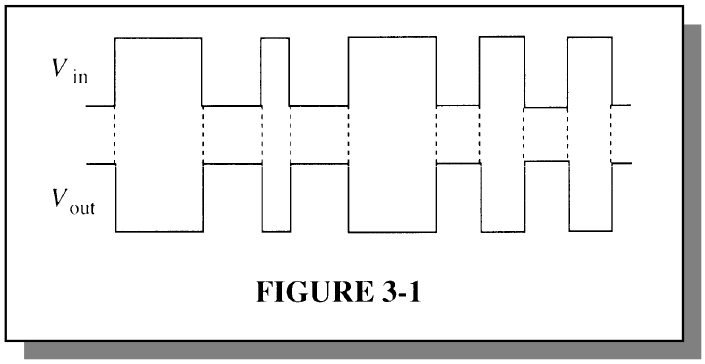
\includegraphics[width=0.33\textwidth]{figures/inv1.png}
\caption{\label{fig:inv1} Solution for Exercise 1.}
\end{figure}
\item Exercise 2: B) LOW C) HIGH D) LOW E) HIGH F) LOW
\end{enumerate}

\section{3-2: The AND Gate}

\begin{enumerate}
\item Exercise 5: See Fig. \ref{fig:and1}.  Notice that $X = B$.
\begin{figure}[ht]
\centering
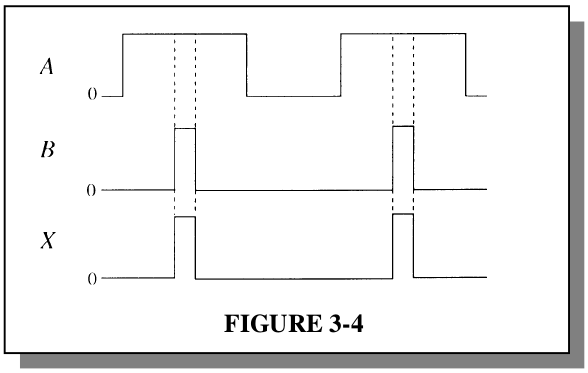
\includegraphics[width=0.33\textwidth]{figures/and1.png}
\caption{\label{fig:and1} Solution for Exercise 5.}
\end{figure}
\item Exercise 7: See Fig. \ref{fig:and2}.  Notice that $X = C$.
\begin{figure}[hb]
\centering
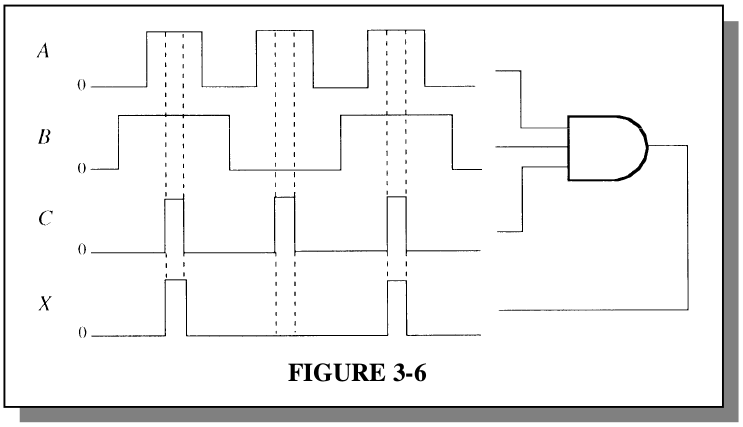
\includegraphics[width=0.33\textwidth]{figures/and2.png}
\caption{\label{fig:and2} Solution for Exercise 7.}
\end{figure}
\end{enumerate}

\clearpage

\section{3-3: The OR Gate}

\begin{enumerate}
\item Exercise 11: See Fig. \ref{fig:or1}.
\begin{figure}[ht]
\centering
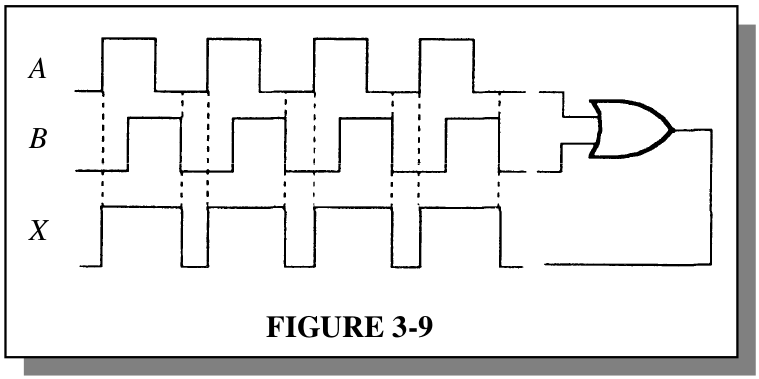
\includegraphics[width=0.33\textwidth]{figures/or1.png}
\caption{\label{fig:or1} Solution for Exercise 11.}
\end{figure}
\item Exercise 12: See Fig. \ref{fig:or2}.
\begin{figure}[ht]
\centering
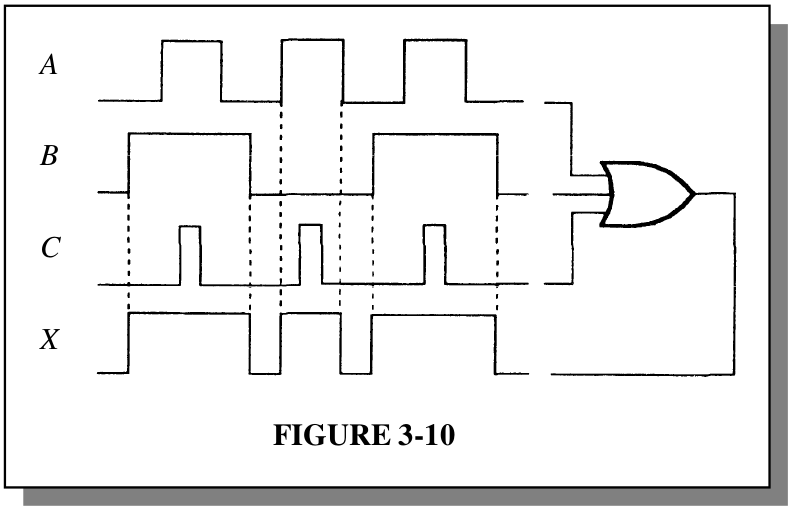
\includegraphics[width=0.33\textwidth]{figures/or2.png}
\caption{\label{fig:or2} Solution for Exercise 12.}
\end{figure}
\item Exercise 14: See Fig. \ref{fig:or3}.
\begin{figure}[ht]
\centering
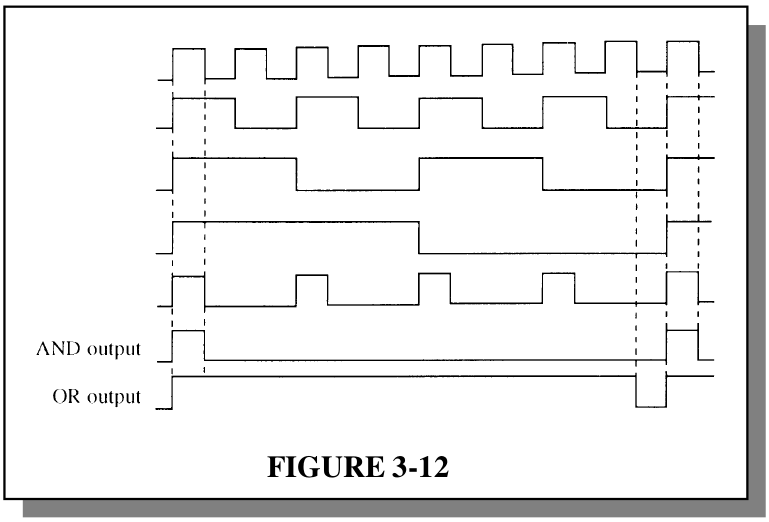
\includegraphics[width=0.33\textwidth]{figures/or3.png}
\caption{\label{fig:or3} Solution for Exercise 14.}
\end{figure}
\end{enumerate}

\section{3-4: The NAND Gate}

\begin{enumerate}
\item Exercise 17: See Fig. \ref{fig:nand1}.  Notice that the output alternates between $\bar{A}$ and $TRUE$.
\begin{figure}[h!]
\centering
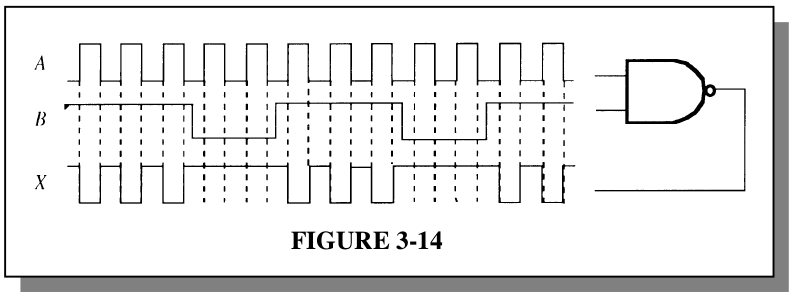
\includegraphics[width=0.33\textwidth]{figures/nand1.png}
\caption{\label{fig:nand1} Solution for Exercise 17.}
\end{figure}
\clearpage
\item Exercise 18: See Fig. \ref{fig:nand2}.  Notice that the output alternates between $\bar{C}$ and $TRUE$.
\begin{figure}[ht]
\centering
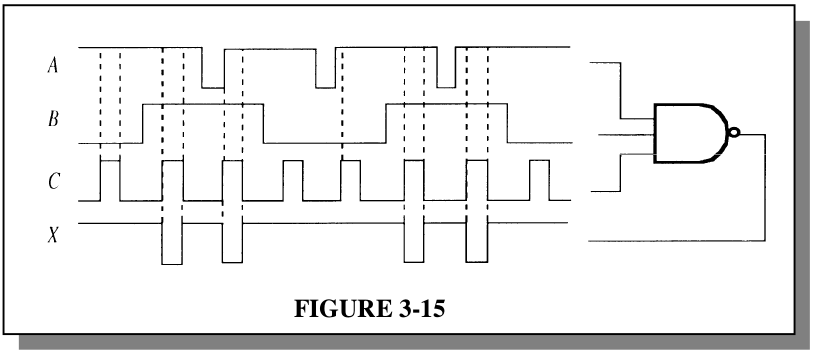
\includegraphics[width=0.33\textwidth]{figures/nand2.png}
\caption{\label{fig:nand2} Solution for Exercise 18.}
\end{figure}
\item Exercise 19: See Fig. \ref{fig:nand3}.  Notice that the output is $LOW$ only when all inputs are high.
\begin{figure}[ht]
\centering
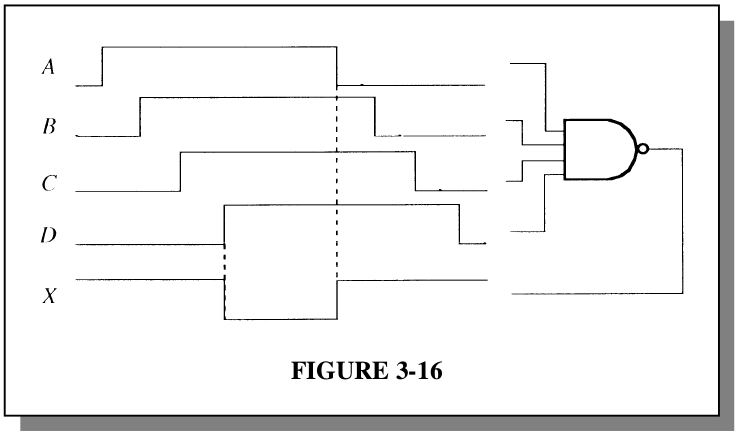
\includegraphics[width=0.33\textwidth]{figures/nand3.png}
\caption{\label{fig:nand3} Solution for Exercise 19.}
\end{figure}
\end{enumerate}

\section{3-6: The Exclusive-OR and Exclusive-NOR Gates}

\begin{enumerate}
\item Exercise 26: See Fig. \ref{fig:xor1}.  Notice that the output alternates between $\bar{A}$ and $A$.
\begin{figure}[ht]
\centering
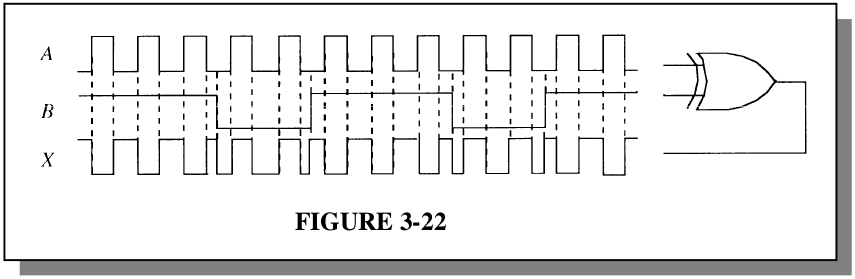
\includegraphics[width=0.5\textwidth]{figures/xor1.png}
\caption{\label{fig:xor1} Solution for Exercise 26.}
\end{figure}
\end{enumerate}

\section{3-7: Programmable Logic}

\begin{enumerate}
\item Exercise 29: The connections imply the following three outputs:
\begin{align}
X_1 &= \bar{A}B \\
X_2 &= \bar{A}\bar{B} \\ 
X_3 &= A\bar{B}
\end{align}
\end{enumerate}

\section{3-9: Troubleshooting}

\begin{enumerate}
\item The gates are faulty in cases (a), (b), and (d).  The gate in case (c) is functioning correctly.
\end{enumerate}

\clearpage

\section{Special Design Problems}

\begin{enumerate}
\item Exercise 47: See Fig. \ref{fig:special}.  I would add Ignition Switch $AND$ Lights Switch, and $XOR$ that output with the timer output.
\begin{figure}[ht]
\centering
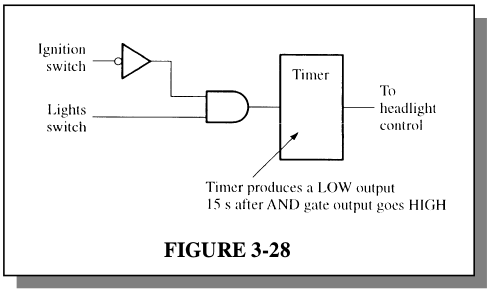
\includegraphics[width=0.33\textwidth]{figures/special.png}
\caption{\label{fig:special} Solution for Exercise 47.}
\end{figure}
\end{enumerate}

\end{document}
